\chapter{Trajectory Optimization}
\label{ch:trajectory_optimization}

\section{From an Impact Task to a Candidate Motion}

A trajectory optimizer answers a conditional question: among the motions
allowed by a specified model and its constraints, which performs best under
a declared objective? For golf, the result might be a candidate downswing
that delivers a desired contact state with limited actuator effort. It is
neither a measured human strategy nor a guarantee that a player can execute
the motion. Those conclusions need additional evidence.

The previous chapters establish the pieces of this question. Configuration
geometry determines how motion and force are represented. Underactuated
dynamics restrict which timed paths are feasible. Transverse and event
analysis explain how perturbations affect a nominal motion and its impact
outcome. Optimization joins these pieces by choosing a feasible reference,
and possibly a feedback policy, under explicit performance and uncertainty
criteria. A reference need not be optimal before it is useful for tracking
or identification.

Let $x$ contain the mechanical state and any required actuator or environmental
states, and let $u$ be the command. For a smooth phase, a deterministic
optimal-control problem can be written
\begin{equation}\label{eq:ocp_cost}
\begin{aligned}
 \min_{x(\cdot),u(\cdot),T}\quad &
 \phi(x(T),T)+\int_0^T L(x(t),u(t),t)\,dt,\\
 \dot x&=f(x,u,t),\qquad x(0)=x_0,\\
 c(x,u,t)&\leq0,\qquad \psi(x(T),T)=0,\\
 0<T_{\min}&\leq T\leq T_{\max}.
\end{aligned}
\end{equation}
Bounds on duration are modeling choices, not mandatory features of every
OCP; they are useful when unlimited waiting or pumping would undermine the
intended task. The initial state, admissible controls, regularity, and event
sequence must be specified. Existence of a minimizer also requires suitable
compactness/coercivity and closure conditions. A nonempty numerical search
space alone does not establish existence or attainability.

A stationary ball can make absolute start time irrelevant in an autonomous
model. Duration still changes acceleration, effort, dissipation, noise
accumulation, and actuator feasibility. A moving ball, gust, imposed rhythm,
or fatigue state introduces further timing dependence. A pause is feasible
only if the full state can be held or evolves admissibly during that pause.
Free final time is permission to optimize timing, not permission to ignore it.

The terminal constraint must encode the actual contact geometry. A scalar
signed gap $h(x,t)=0$ can describe an impact guard, while additional target
conditions describe strike location, face orientation, and other outputs.
Not every equality in $\psi$ is an event guard. For first passage, require
no earlier contact and the chosen crossing direction; at a regular event,
$h_t+h_xf\ne0$. A terminal equality alone could select a later crossing or
an approach from the wrong side. Finite face and ball geometry, rather than
coincidence of idealized centers, should define a physical collision model.

If post-impact ball speed or dispersion is the objective, include the impact
map and any subsequent flight model needed to compute that outcome. Pre-impact
clubhead speed is a proxy that omits strike location, orientation, restitution,
friction, and equipment deformation. Acceleration at the endpoint is likewise
not automatically a useful impact objective. Select quantities because the
model and evidence connect them to the question being investigated.

\section{Timing, Effort, and Well-Posed Objectives}

Consider the nondimensional integrator $\dot q=u$, with $q(0)=0$, $q(T)=D>0$,
and cost $\tfrac12\int_0^T u^2dt$. Cauchy--Schwarz gives
\begin{equation}\label{eq:free_time_effort}
 D^2=\left(\int_0^T u\,dt\right)^2
 \leq T\int_0^T u^2dt,\qquad
 J_{\min}(T)=\frac{D^2}{2T},\quad u_*=D/T.
\end{equation}
With unrestricted $T$, the infimum is zero as $T\to\infty$ and is not attained
at finite duration. Adding $\rho T$, $\rho>0$, gives
$T_*=D/\sqrt{2\rho}$ if no other constraint is active. This simple example
shows why a free-time objective needs scrutiny before choosing a solver.

A quadratic torque penalty is a weighted effort surrogate. It is not
mechanical work: actuator power is $u^T\dot q_a$ for work-conjugate actuator
coordinates, and positive/negative work, heat, activation, and fatigue require
their own models. Cost weights have units that make the summed terms
commensurate, or the variables should be explicitly nondimensionalized.
Changing those scales changes the question unless the weights transform too.
Low commanded torque does not by itself ensure low muscle force or repeatability.

For a fixed-duration rest-to-rest double integrator,
$\dot q=v$, $\dot v=u$, the minimum of $\tfrac12\int u^2dt$ with
$(q,v)(0)=(0,0)$ and $(q,v)(T)=(D,0)$ is
\begin{equation}\label{eq:cubic_optimal_motion}
 \begin{aligned}
 s&=t/T,\qquad q_*=D(3s^2-2s^3),\\
 v_*&=(6D/T)(s-s^2),\qquad
 u_*=(6D/T^2)(1-2s),\qquad J_*=6D^2/T^3.
 \end{aligned}
\end{equation}
The stationarity condition makes $u$ affine in time; the two integral endpoint
conditions determine its coefficients. The strictly convex quadratic cost
and linear constraints make this the unique minimizing control up to
changes on sets of measure zero. An acceleration bound $|u|\leq a$ is
satisfied by this solution only if $6D/T^2\leq a$.

Changing the same plant's objective changes its control. Minimum-time
rest-to-rest travel with $|u|\leq a$ uses $+a$ followed by $-a$, with
$T=2\sqrt{D/a}$. For monotone first passage to $q=D$ from rest with terminal
velocity free, maximum arrival speed under the same acceleration bound is
$v(T)=\sqrt{2aD}$, achieved by $u=+a$ throughout and
$T=\sqrt{2D/a}$. Indeed, $v(T)^2=2\int_0^D u\,dq\leq2aD$.
The monotonicity and first-passage assumptions matter. These are calculated
particle examples, not golf optimizations. They demonstrate why a torque
reversal cannot be inferred without specifying the task and constraints.

\begin{figure}[htbp]
\centering
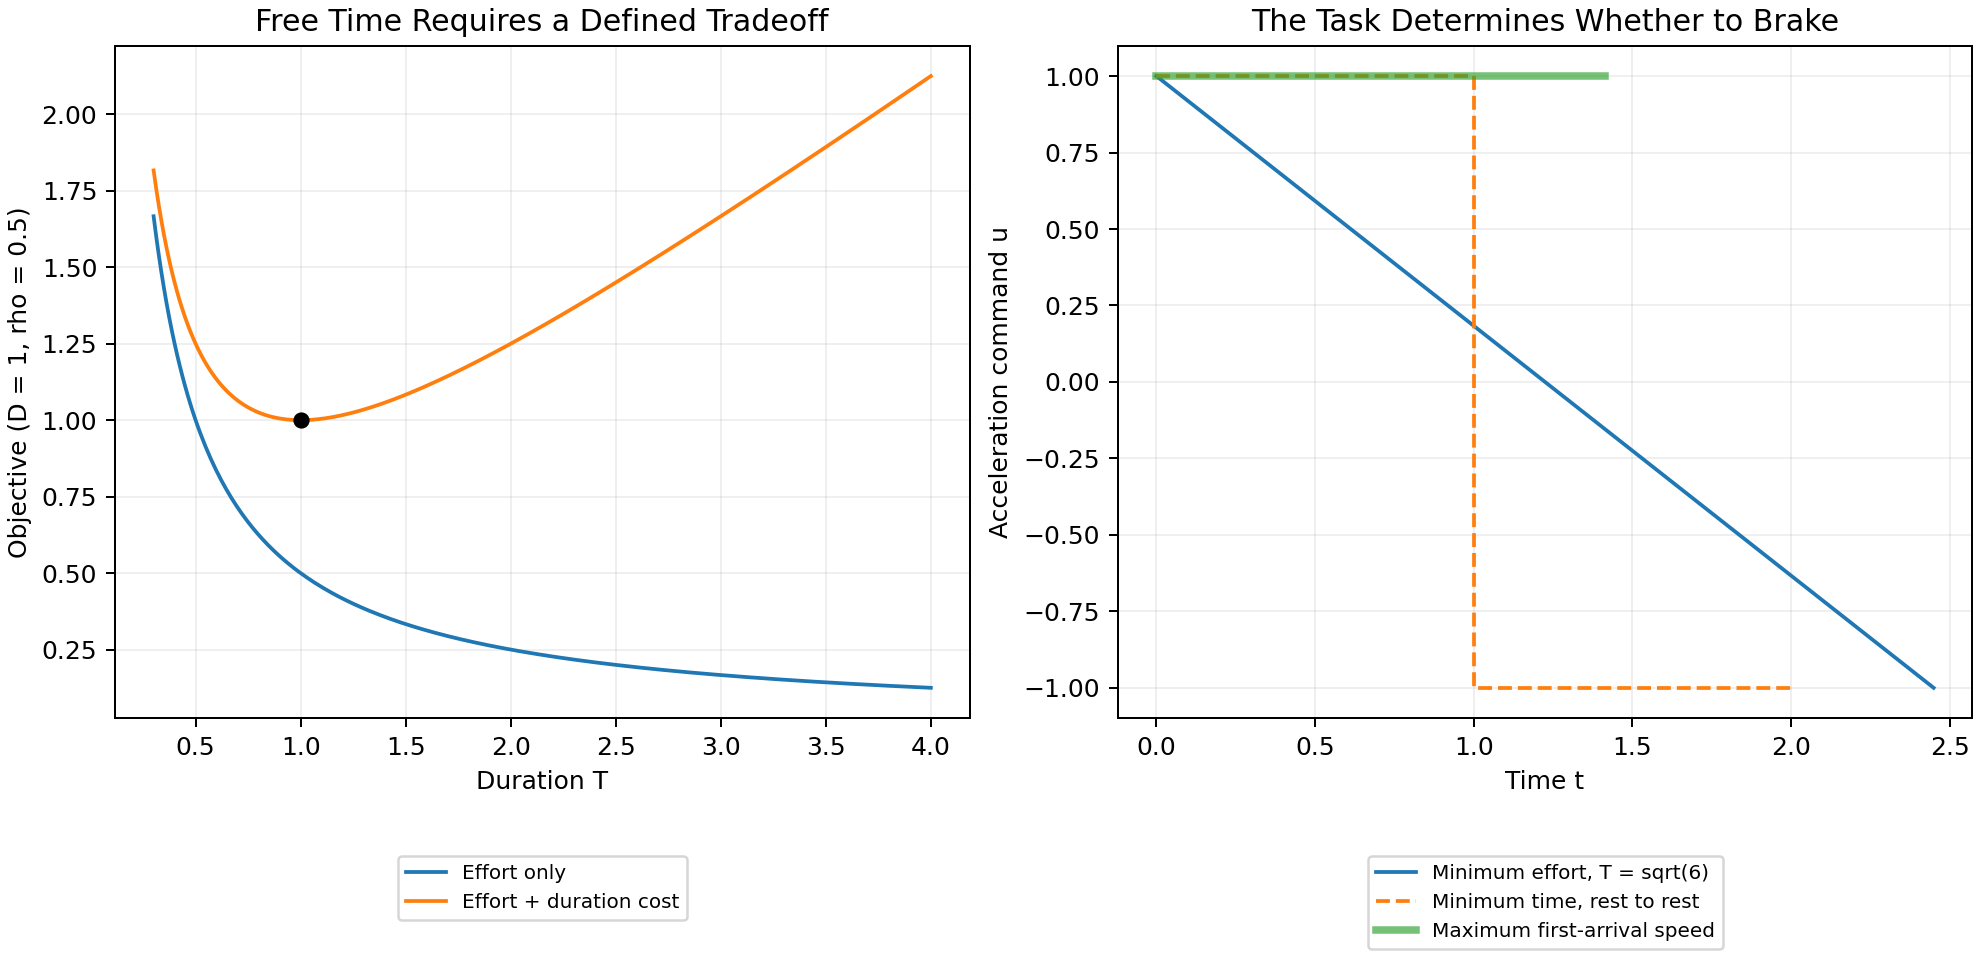
\includegraphics[width=\linewidth]{../figures/trajectory_objective_comparison.png}
\caption{Different Objectives Select Different Controls}
\label{fig:trajectory_objective_comparison}
\end{figure}
The left panel uses the integrator with $D=1$ and $\rho=0.5$. The right
uses the double integrator with $D=1$ and $|u|\leq1$: the effort-minimizing
rest-to-rest example has $T=\sqrt6$, the minimum-time rest-to-rest example
has $T=2$, and maximum first-arrival speed uses $T=\sqrt2$. Their different
endpoint and duration requirements explain the different controls.

\section{Necessary Conditions and Hamiltonian Conventions}

On a smooth unconstrained arc of a normal extremal, use the minimization
convention
\begin{equation}\label{eq:ocp_hamiltonian}
 \mathcal H=L+p^Tf,\qquad
 \dot p=-\mathcal H_x,\qquad
 u_*\in\operatorname*{arg\,min}_{u\in\mathcal U}\mathcal H(x_*,u,p,t).
\end{equation}
Here gradients in the costate equation are columns. For regular terminal
equalities, there is a multiplier $\nu$ such that
\begin{equation}\label{eq:ocp_transversality}
 p(T)=\phi_x+\psi_x^T\nu,\qquad
 \mathcal H(T)+\phi_T+\nu^T\psi_T=0.
\end{equation}
The second condition applies to an interior free final time; it is absent
for fixed time and is modified at an active time bound. Endpoint derivatives
hold $x$ fixed. State/path constraints require their own multipliers and
possibly junction conditions; the displayed unconstrained adjoint is not a
complete formula for contact or state-constrained arcs. Abnormal extremals
cannot normalize the running-cost multiplier to one and need the general
maximum/minimum principle.

The alternative maximum convention uses a consistently transformed costate
and Hamiltonian, commonly $\tilde p^Tf-L$. Maximizing $L+p^Tf$ with the
minimization costate equations reverses the control selection. For
$L=u^2/2$ and $f=u$, minimization gives $u=-p$; maximization over unbounded
$u$ has no finite solution. In an autonomous free-time problem without
explicit endpoint-time dependence, the normal Hamiltonian is zero along
the optimum on the applicable smooth arcs. A fixed-time problem does not
inherit that zero condition.

These are necessary conditions under the relevant assumptions, not a general
certificate of global optimality. If the Hamiltonian is affine in a bounded
scalar input, a nonzero switching coefficient selects a bound. If that
coefficient vanishes over an interval, higher-order conditions may determine
a singular arc. Quadratic effort, actuator dynamics, rate constraints, or
active state constraints change this structure. A smooth wrist release does
not identify a singular optimal-control arc or a pattern of muscle activation.

\section{Transcription and Numerical Verification}

Use normalized time $s=t/T\in[0,1]$. The chain rule and change of variables give
\begin{equation}\label{eq:normalized_ocp}
 \frac{dx}{ds}=T f(x,u,Ts),\qquad
 J=\phi(x(1),T)+T\int_0^1 L(x(s),u(s),Ts)\,ds.
\end{equation}
Thus a constant physical speed $f=2$ over $T=3$ gives $dx/ds=6$.
Multiplying $dx/ds$ by $T$ instead would give the wrong physical duration.
Both dynamics and objective must carry the same consistent scaling.

The numerical decision vector contains state samples, control parameters,
possibly duration and policy parameters, and any algebraic variables. Write
equalities and inequalities separately. Scale residuals by meaningful state,
force, and time scales; a solver tolerance is otherwise difficult to interpret.
Derivatives must include the dependence on $T$ and on event or reset variables.

\subsection{Shooting and Collocation}

Multiple shooting introduces interval initial states and enforces
$x_{k+1}-\widehat\Phi_k(x_k,u_k,T)=0$, where $\widehat\Phi_k$ is a numerical
flow map for the declared control parameterization. Shorter integrations
and sparse continuity constraints often improve conditioning relative to
single shooting. They do not remove physical instability, guarantee convergence,
or make integration error vanish. Matching the numerical map to solver
tolerance is different from matching the exact differential equation.

Direct collocation represents states and controls by chosen polynomials
and imposes dynamics at selected points. One concrete Hermite--Simpson
interval, of physical duration $h_k=T(s_{k+1}-s_k)$, uses
\begin{equation}\label{eq:hermite_simpson}
 \begin{aligned}
 x_c&=\tfrac12(x_k+x_{k+1})+\tfrac{h_k}{8}(f_k-f_{k+1}),\\
 0&=x_{k+1}-x_k-\tfrac{h_k}{6}(f_k+4f_c+f_{k+1}).
 \end{aligned}
\end{equation}
Here $f_c=f(x_c,u_c,t_c)$ and, for a linearly interpolated control,
$u_c=(u_k+u_{k+1})/2$. A cubic Hermite state interpolant has the endpoint
derivatives $f_k,f_{k+1}$; its midpoint derivative condition yields the defect
above. Use a matching quadrature rule for the cost. Smoothness and interpolation
choices determine accuracy; not every collocation method uses these polynomials.

For the rest-to-rest cubic example with $D=1,T=2$, the endpoint states are
$(0,0)$ and $(1,0)$, and accelerations are $1.5$ and $-1.5$. These formulas
give $x_c=(0.5,0.75)$ and zero Simpson defect. That exact polynomial check
is a useful unit test before applying transcription to multibody dynamics.

\subsection{What Solver Success Does Not Establish}

Dynamics enforced at finitely many points need not hold between them. For
example, a residual proportional to $s(s-1/2)(s-1)$ vanishes at three sample
points and is nonzero elsewhere. A path $q(s)=4s(1-s)$ satisfies
$q\leq1/2$ at its endpoints and violates it at the midpoint. Checking a few
additional points reduces the risk of missing such behavior but is not a
continuous-interval proof.

Reintegrate the optimized control with an independent, tighter error-controlled
solver, preserving its actual interpolation and the same initial state.
Compare the resulting path, first event, terminal outputs, and constraints
with the transcription. Inspect differential residuals between nodes and
repeat on refined meshes until the quantities of interest stabilize to stated
tolerances. Integration agreement supports numerical fidelity to the model;
it does not validate the model itself. A rigorous continuous-time certificate
requires additional bounds on residuals, interpolation, and constraint margins.

Nonconvex solvers may find different feasible local solutions from different
initial guesses, or return an infeasible stationary point. Report termination
status, primal residuals, stationarity measures, active bounds, discretization,
and results across starts. Use a finite stopping budget and return failure
when acceptance criteria are unmet. Relaxing a constraint for continuation
is useful only if the original constraint is restored and checked before
accepting the result. No algorithmic workflow should promise a feasible
trajectory for an infeasible problem.

\section{Mechanics and Clubhead Speed}

For minimal mechanical coordinates $q$, write
\begin{equation}\label{eq:ocp_underactuation}
 \dot q=v,\qquad M(q)\dot v+b(q,v)=B(q)u+F_{\rm ext}(q,v,t).
\end{equation}
The bias $b$ includes the chosen velocity, potential, and passive terms once.
The state is $x=(q,v)$, possibly augmented; $M$ acts on configuration
accelerations, not on a second derivative of the entire state. On a regular
patch, a left annihilator $N_BB=0$ gives
$N_B(M\dot v+b-F_{\rm ext})=0$. This tests membership in the unrestricted
actuation image. Input magnitude/rate limits and actuator states remain
separate constraints. A correct first-order transcription already enforces
these passive equations, so adding a redundant annihilator constraint is
not generally necessary.

For closed chains or maintained contacts, include the independent closure
constraints, compatible velocities, and constraint reactions or use a valid
minimal-coordinate reduction. Ideal reactions can exert force without doing
work along an admissible velocity. Unilateral contact also requires the
appropriate nonpenetration, reaction-sign, friction, and mode conditions.
An optimizer that ignores these conditions can obtain an attractive objective
from a mechanically impossible motion. Contact switches need separate phases
and reset/guard constraints, or a contact formulation whose approximation
and convergence are explicitly assessed.

If the clubhead point is $r(q)$, its velocity is $J_r(q)v$ and its speed is
$\|J_rv\|$. With the absolute planar angles of Chapter 5,
\begin{equation}\label{eq:ocp_clubhead_speed}
 \|\dot r\|^2=l_1^2\dot\theta_1^2+l_2^2\dot\theta_2^2
 +2l_1l_2\cos(\theta_1-\theta_2)\dot\theta_1\dot\theta_2.
\end{equation}
For aligned unit links and $\dot\theta_2=1$, changing $\dot\theta_1$ from
$-1$ to $1$ changes tip speed from zero to two. Distal angular velocity
alone therefore does not determine linear clubhead speed. A moving shoulder,
distributed shaft deformation, and a different angle convention require the
corresponding kinematics rather than this particular two-link formula.

The passive club equation relates arm acceleration, coupling, gravity, and
velocity terms. It does not specify the sign of shoulder torque or an
optimal switching schedule. A credible golf optimization must publish its
parameters, initial state, objective, input bounds, contact conditions, and
converged solution before describing such a schedule as a result. Compare
alternative objectives and model assumptions, and inspect whole-system
and segment energy/power balances to explain the mechanism. A nominal
simulation is not evidence that a player should actively brake a segment.

\section{Repeatability Requires an Uncertainty Model}

Separate initial-state variation, uncertain parameters, disturbances, motor
command variability, observation noise, and feedback/estimation errors.
They enter different equations and can have different time correlations.
A single Gaussian random vector can model a random initial condition or a
finite set of uncertain parameters. It is not automatically a continuous
noise process, nor signal-dependent noise merely because its covariance is
named in the objective.

Harris and Wolpert's 1998 theory investigated eye and goal-directed arm
movements using signal-dependent neural-command noise. It motivates a class
of hypotheses; it does not supply a universal golf joint-torque noise law.
Torque is already the result of activation and muscle mechanics. A chosen
model such as conditional command covariance proportional to $u_j^2$ needs
calibration, units, sampling interval, correlation structure, and validation
for the intended movement.

For a local discrete linear model with feedback
$u=u_*-K_k\delta x$, independent zero-mean noise $w_k$ of identity covariance,
and $\delta x_{k+1}=A_{{\rm cl},k}\delta x_k+G_kw_k$, covariance satisfies
\begin{equation}\label{eq:ocp_covariance}
 A_{{\rm cl},k}=A_k-B_kK_k,\qquad
 \Sigma_{k+1}=A_{{\rm cl},k}\Sigma_kA_{{\rm cl},k}^T+G_kG_k^T.
\end{equation}
This is exact for the stated linear model. Substituting Jacobians and nominal
diffusion amplitudes from nonlinear dynamics gives a local approximation.
Covariance propagation alone is analysis; covariance steering additionally
chooses admissible controls or policies to meet distributional objectives
or constraints. Neither phrase identifies a biological controller.

Freezing signal-dependent diffusion at its nominal value can omit
multiplicative terms. For the zero-mean scalar example
$\xi_{k+1}=a\xi_k+n\xi_kw_k+g w_k$, with $w_k$ independent of $\xi_k$,
\begin{equation}\label{eq:multiplicative_covariance}
 \Sigma_{k+1}=(a^2+n^2)\Sigma_k+g^2.
\end{equation}
The $n^2\Sigma_k$ term survives even though the state mean is zero. With
$a=0.5,n=0.2,g=0.1,\Sigma_k=1$, the next variance is $0.30$, compared with
$0.26$ if multiplicative noise is discarded. Correlated or colored noise
requires the corresponding cross-covariances or augmented dynamics. State
and diffusion linearizations must therefore be described, not silently
replaced with an additive-noise formula.

\section{Impact Loss, Sensitivity, and Risk}

Let $y$ be a physically scaled impact outcome, not just the terminal guard
residual. For a random output with mean $\mu_y$
and covariance $\Sigma_y$, a quadratic loss satisfies
\begin{equation}\label{eq:ocp_output_loss}
 \mathbb E[(y-y_d)^TW(y-y_d)]
 =(\mu_y-y_d)^TW(\mu_y-y_d)+\operatorname{tr}(W\Sigma_y),
 \qquad W\succeq0.
\end{equation}
This identity only needs finite second moments. Penalizing covariance alone
can favor a repeatable miss. Combining mean outcome, dispersion, effort, and
constraint risk with declared weights makes the tradeoffs explicit. For a
nonquadratic expected cost, the mean trajectory alone generally does not
determine the expectation.

At an event, Chapter 4 gives the output sensitivity to a fixed-time state
perturbation just before the nominal event:
\begin{equation}\label{eq:ocp_event_output}
 C_e=H_x-\frac{(H_xf+H_t)h_x}{h_t+h_xf},\qquad
 \Sigma_y\approx C_e\Sigma^-C_e^T.
\end{equation}
Here $y=H(x,t)$ is a smooth pre-event output and $h=0$ is the regular guard.
The approximation assumes small perturbations and the same event sequence;
parameter/measurement uncertainty and cross-covariances add further terms.
If post-impact states are compared at a common time, use the reset and
saltation map from Chapter 4. Near grazing or changing contact order, these
local derivatives can fail.

For an actual hitting event, $h(x(t_e),t_e)=0$ by definition for trajectories
that hit it. Its variance does not measure all strike errors, and trajectories
that never hit require a separate failure outcome. Propagate the relevant
face, location, velocity, and ball-flight outputs instead. The condition
number of $\psi_x$ is also not an absolute error-amplification measure:
$I$ and $1000I$ both have condition number one but their gains differ by
a factor of one thousand. The dynamics-to-event map, physical metrics,
input uncertainty, and singular values determine local output sensitivity.

A Gaussian scalar approximation to a one-sided chance constraint
$a^Tx\leq b$ gives
\begin{equation}\label{eq:ocp_chance_constraint}
 a^T\mu+\Phi_{\rm N}^{-1}(1-\epsilon)
 \sqrt{a^T\Sigma a}\leq b.
\end{equation}
Here $\Phi_{\rm N}$ is the standard normal distribution function. This is a
marginal probability statement under the specified distribution, not a
guarantee for every state or every time. Ten independent constraints each
met with probability $0.95$ have joint success probability $0.95^{10}$,
about $0.599$. Allocating failure probabilities whose sum is at most a
target $\epsilon$ gives a conservative union-bound guarantee for the finite
collection, without requiring independence. Continuous-time safety still
needs treatment between the checked times. Gaussian models have unbounded
tails and cannot provide deterministic hard bounds on every realization.

Local covariance analysis is not a robustness certificate for the nonlinear
swing. Validate predicted means, tails, event failures, and constraint
violations with independent simulations and held-out measurements, reporting
sampling uncertainty. Worst-case bounded-disturbance verification answers
a different question and requires the set-invariance conditions of the
funnel chapter. A stochastic objective may favor lower effort, a different
reference, or stronger active feedback; it need not select passive stability,
submaximal speed, or a geometrically wider funnel.

\section{Search, Comparison, and Scientific Interpretation}

Derivative-free population methods can explore policy parameters and provide
warm starts when derivatives are unavailable or unreliable. Gradient-based
methods can exploit sparse derivatives for local refinement. Neither a
population search nor multiple initial guesses guarantees a global solution
to a nonconvex swing problem. Contact events do not make derivatives
universally unavailable: regular event sensitivities may be computed, while
mode changes and grazing require special care. State the actual derivative
and contact treatment.

For an equality-constrained task, rejecting every inexact candidate may leave
no feasible population. Use a feasibility-preserving parameterization,
constraint restoration, or a documented tolerance, and return an explicit
failure if no acceptable candidate exists. Penalties and relaxed constraints
must not silently redefine the final task. Report computational effort and
best feasible objectives, not an unqualified claim of global discovery.

A useful golf comparison holds the task and admissible mechanics fixed while
changing one proposed explanation: input distribution, timing, feedback,
equipment parameters, or uncertainty model. Check whether the result
persists across parameter uncertainty, meshes, initial guesses, and held-out
trials. If several objectives reproduce the same nominal motion, observation
alone does not identify which objective a human optimizes. Forward
interventions and measurable impact predictions can distinguish them.

The output of this chapter is therefore a documented candidate trajectory
and, when optimized, a realizable policy with quantified numerical and
statistical limits. Its geometry, power flow, transient response, and impact
distribution should form one consistent argument. The next chapter asks
which neighborhood can be verified for the chosen nonlinear model and
controller; that neighborhood cannot be assumed from optimizer success.

\section{Further Reading}

\href{https://underactuated.mit.edu/trajopt.html}{Tedrake's trajectory-optimization
notes} compare shooting and transcription. \href{https://arxiv.org/abs/1707.00284}{Kelly's
transcription tutorial} explains numerical and hybrid formulations.
\href{https://liberzon.csl.illinois.edu/teaching/cvoc/node1.html}{Liberzon's
optimal-control text} develops the maximum principle, transversality,
existence, and the distinction between necessary and sufficient conditions;
translate its Hamiltonian convention consistently.
\href{https://underactuated.mit.edu/robust.html}{Tedrake's robust/stochastic
notes} distinguish probabilistic and bounded-disturbance problems.
\href{https://www.nature.com/articles/29528}{Harris and Wolpert's original
noise-model paper} provides the specific motor-planning hypothesis discussed
above, with its original movement scope.

\section{Exercises}

\begin{enumerate}[itemsep=3pt,parsep=0pt]
\item Derive both normalized-time equations. Test them on constant speed
over a duration different from one. State the units of every cost weight.
\item Verify the free-time integrator infimum, then add duration cost and
an input bound. Identify when the bound changes the optimal duration.
\item Derive the rest-to-rest cubic and its effort. Compare its control
with the two bounded-acceleration objectives in the text.
\item Derive the normal PMP conditions using the stated minimum convention.
Explain what changes at fixed terminal time and active path constraints.
\item Check the Hermite--Simpson cubic example, then exhibit an inter-node
constraint violation despite feasible nodes. Propose a verification protocol.
\item Derive clubhead speed in absolute and relative joint angles, including
a moving shoulder. Explain why distal angular speed is insufficient.
\item Compute the multiplicative-noise variance example by averaging over
independent values $\xi,w\in\{-1,1\}$. Compare with the additive approximation.
\item Derive the quadratic output-loss identity and event covariance map.
Explain why variance of an exactly satisfied hitting guard is inadequate.
\item Compare marginal and joint chance constraints. State which assumptions
would allow a statistical claim about continuous-time constraint violations.
\item Specify a reproducible golf optimization and a forward intervention
that could falsify its proposed mechanical explanation. Separate numerical
convergence, model fidelity, repeatability, and human-policy identification.
\end{enumerate}
